%\ctparttext{\color{black}\begin{center}
%		Esta es una descripción de la parte de informática.
%\end{center}}

%\part{Parte de informática}
\chapter{Caso 1: Personas con renta procedente de un alquiler}

\section{Descripción del caso de estudio}
En este caso de estudio se ha elegido el subconjunto con renta neta procedente del alquiler de una
propiedad o terreno en el año anterior al de encuesta mayor que 0 y cualquier régimen de tenencia de la vivienda distinto a cesión gratuita, esto es, en propiedad con o sin hipoteca y en alquiler o realquier en precio normal o inferior al de mercado.

Mediante este caso de estudio se pretende estudiar los gastos, renta e impuestos de las personas que tienen en alquiler algún terreno, para comprobar si la creencia popular sobre si las personas con alquileres tienen mayor poder adquisitivo y más comodidades.

Las variables que se van a seleccionar para realizar el análisis son:
\begin{itemize}
\item \textbf{Renta}: Renta disponible total del hogar en el año anterior al de encuesta.
\item \textbf{Gastos}: Gastos de la vivienda: Alquiler (si la vivienda se encuentra en régimen de alquiler), intereses de la hipoteca (para viviendas en propiedad con pagos pendientes) y otros gastos asociados (comunidad, agua, electricidad, gas, etc.).
\item \textbf{Alimentacion in}: Durante el mes pasado, ¿cuál fue aproximadamente el importe que el hogar gastó en alimentos y bebidas no alcohólicas para ser consumidas en casa?
\item \textbf{IRPF}:Devoluciones/ingresos complementarios por ajustes en impuestos en el año anterior al de encuesta (declaración del IRPF).
\end{itemize}

Este caso de estudio consta de $2292$ respuestas a la encuesta, cada una con las $4$ variables indicadas.

\section{Ejecución de algoritmos}

Ejecutamos ahora la primera celda del notebook de jupyter (que se puede configurar para sacar las distintas gráficas) y obtenemos así las diferentes medidas obtenidas para cada algoritmo, que se muestran en \eqref{tab:c1_alg}.

\begin{table}[H]
\centering
\caption{Caso 1 - Resultados de ejecución de algoritmos.}
\label{tab:c1_alg}
\begin{tabular}{ccccc}
\toprule
 Algoritmo & Tiempo (s) & Calinski-Harabasz & Silhouette & Número de clusters \\
\midrule
kmeans & 0.057 & 625.999 & 0.33432 & 5 \\
birch & 0.106 & 336.711 & 0.48426 & 5 \\
spectral & 0.646 & 534.083 & 0.29880 & 5 \\
dbscan & 0.126 & 333.456 & 0.67367 & 2 \\
meanshift & 10.410 & 73.801 & 0.35908 & 32 \\
\bottomrule
\end{tabular}
\end{table}

En primer lugar, nos llama la atención que spectral cluster es el segundo algoritmo que más ha tardado en su ejecucución, pese a que no ha obtenido (a simple vista y basándonos solo en los resultados mostrados en la tabla) mejores resultados que otros algoritmos. El algoritmo más lento ha sido meanshift, lo que puede deberse a tener que calcular el bandwith, que es una operación costosa.

También es destacable como DBSCAN ha generado solamente 2 clusters, donde uno de ellos contiene el $97.21\%$ de los objetos, y el resto se encuentran en el cluster $-1$. Esto causa que su silhouette sea mucho mayor que el del resto de algoritmos.

Observamos además que meanshift ha generado $32$ clusters y ha obtenido el valor de Calinski-Harabasz más bajo de todos. Observando los tamaños de los clusters que ha generado meanshift vemos que uno contiene el $90.66\%$ de los datos, muchos de ellos contienen un solo elemento ($0.04\%$ de los datos totales) y ninguno de los restantes supera el $2\%$ de los datos totales. Podemos concluir por tanto que meanshift no ha hecho un buen agrupamiento.

Los algoritmos kmeans, birch y spectral cluster han obtenido resultados similares, siendo birch el que ha obtenido mejor silhouette, aunque esto puede no ser muy representativo, ya que es una medida muy sensible a la separación de los clusters. Por tanto, nos fijamos de nuevo en Calinski-Harabasz, donde kmeans y spectral cluster han conseguido mejores resultados.


\section{Análisis}


Para el análisis se va a usar spectral cluster, ya que ha obtenido unos resultados aceptables en las medidas. Este algoritmo genera 5 clusters. uno de tamaño mayor y el resto de tamaños similares, como se puede ver en \eqref{c1_tam}

\begin{figure}[H]
\caption{Caso 1- Tamaño de los clusters generados por spectral cluster}
\label{c1_tam}
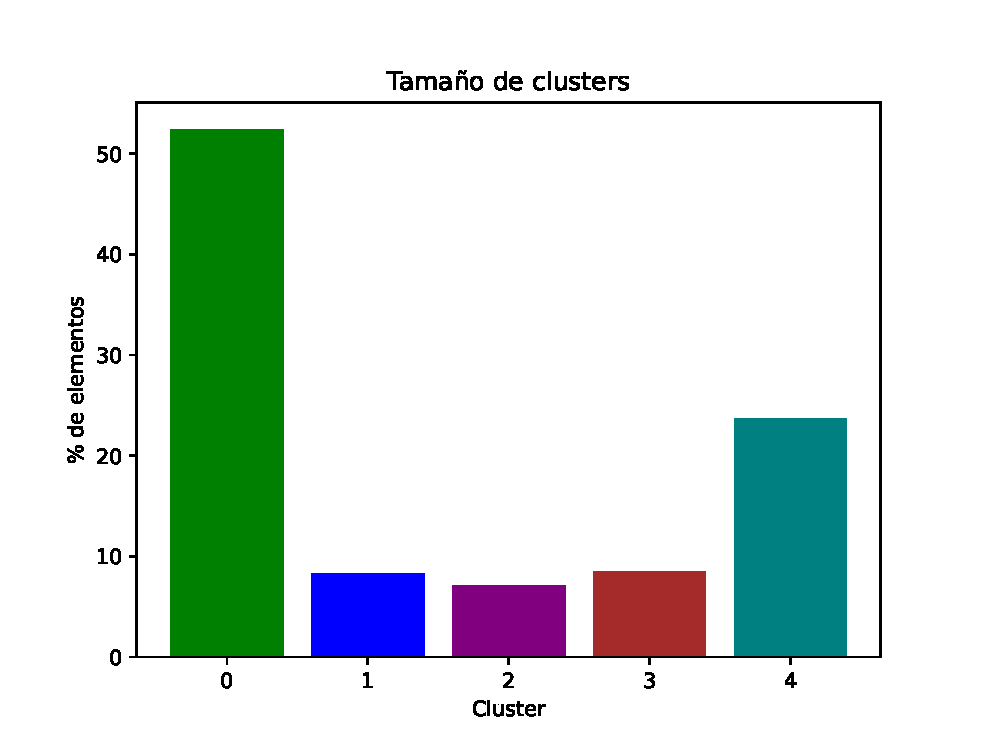
\includegraphics[scale=1]{caso1/spectral/bar.eps}
\end{figure}

A continuación observamos la scatter matrix \eqref{c1_scatter}, donde se puede apreciar como se separan los clusters y qué variables son necesarias para separar cada uno.

\begin{figure}[H]
\caption{Caso 1- Scatter matrix de spectral cluster}
\label{c1_scatter}
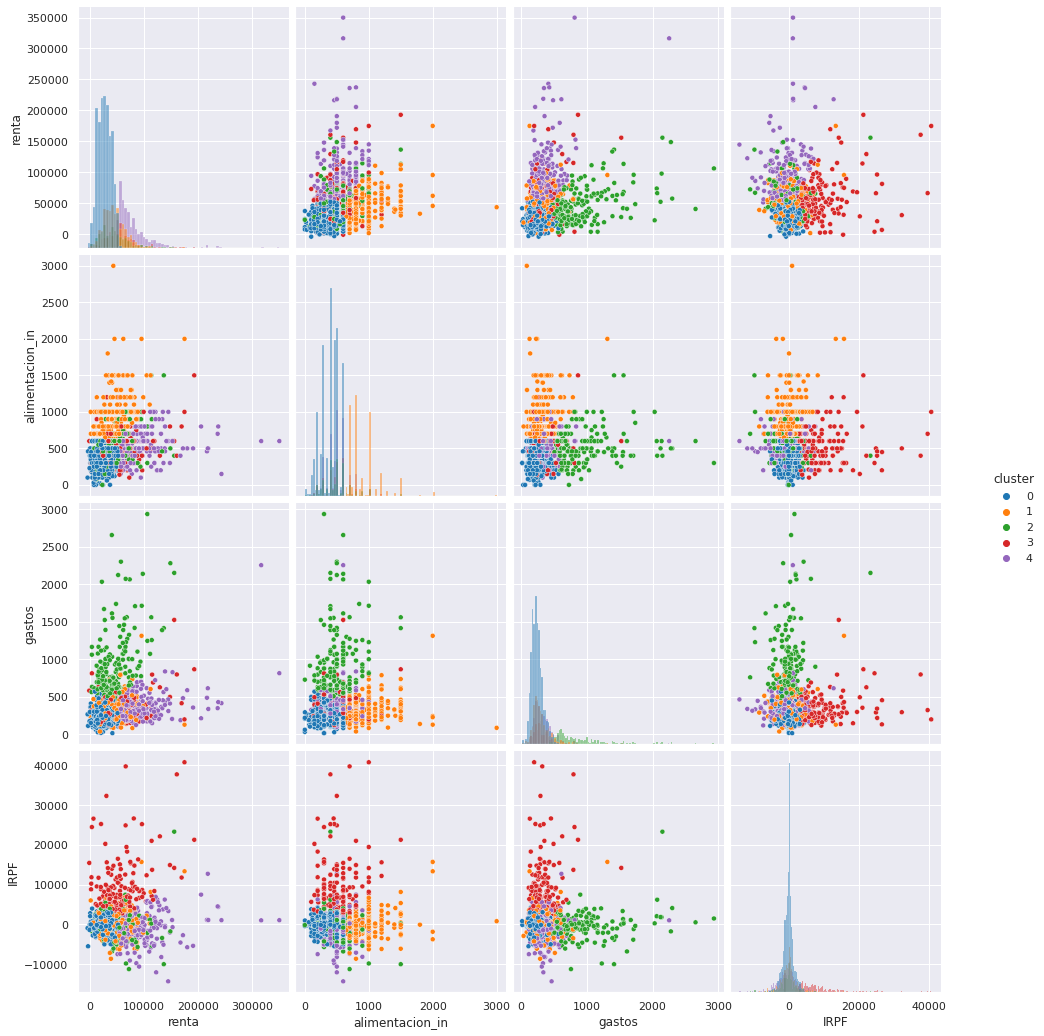
\includegraphics[scale=0.45]{caso1/spectral/scatter.png}
\end{figure}


\begin{figure}[H]
\caption{Caso 1- Boxplot de spectral cluster}
\label{c1_boxplot}
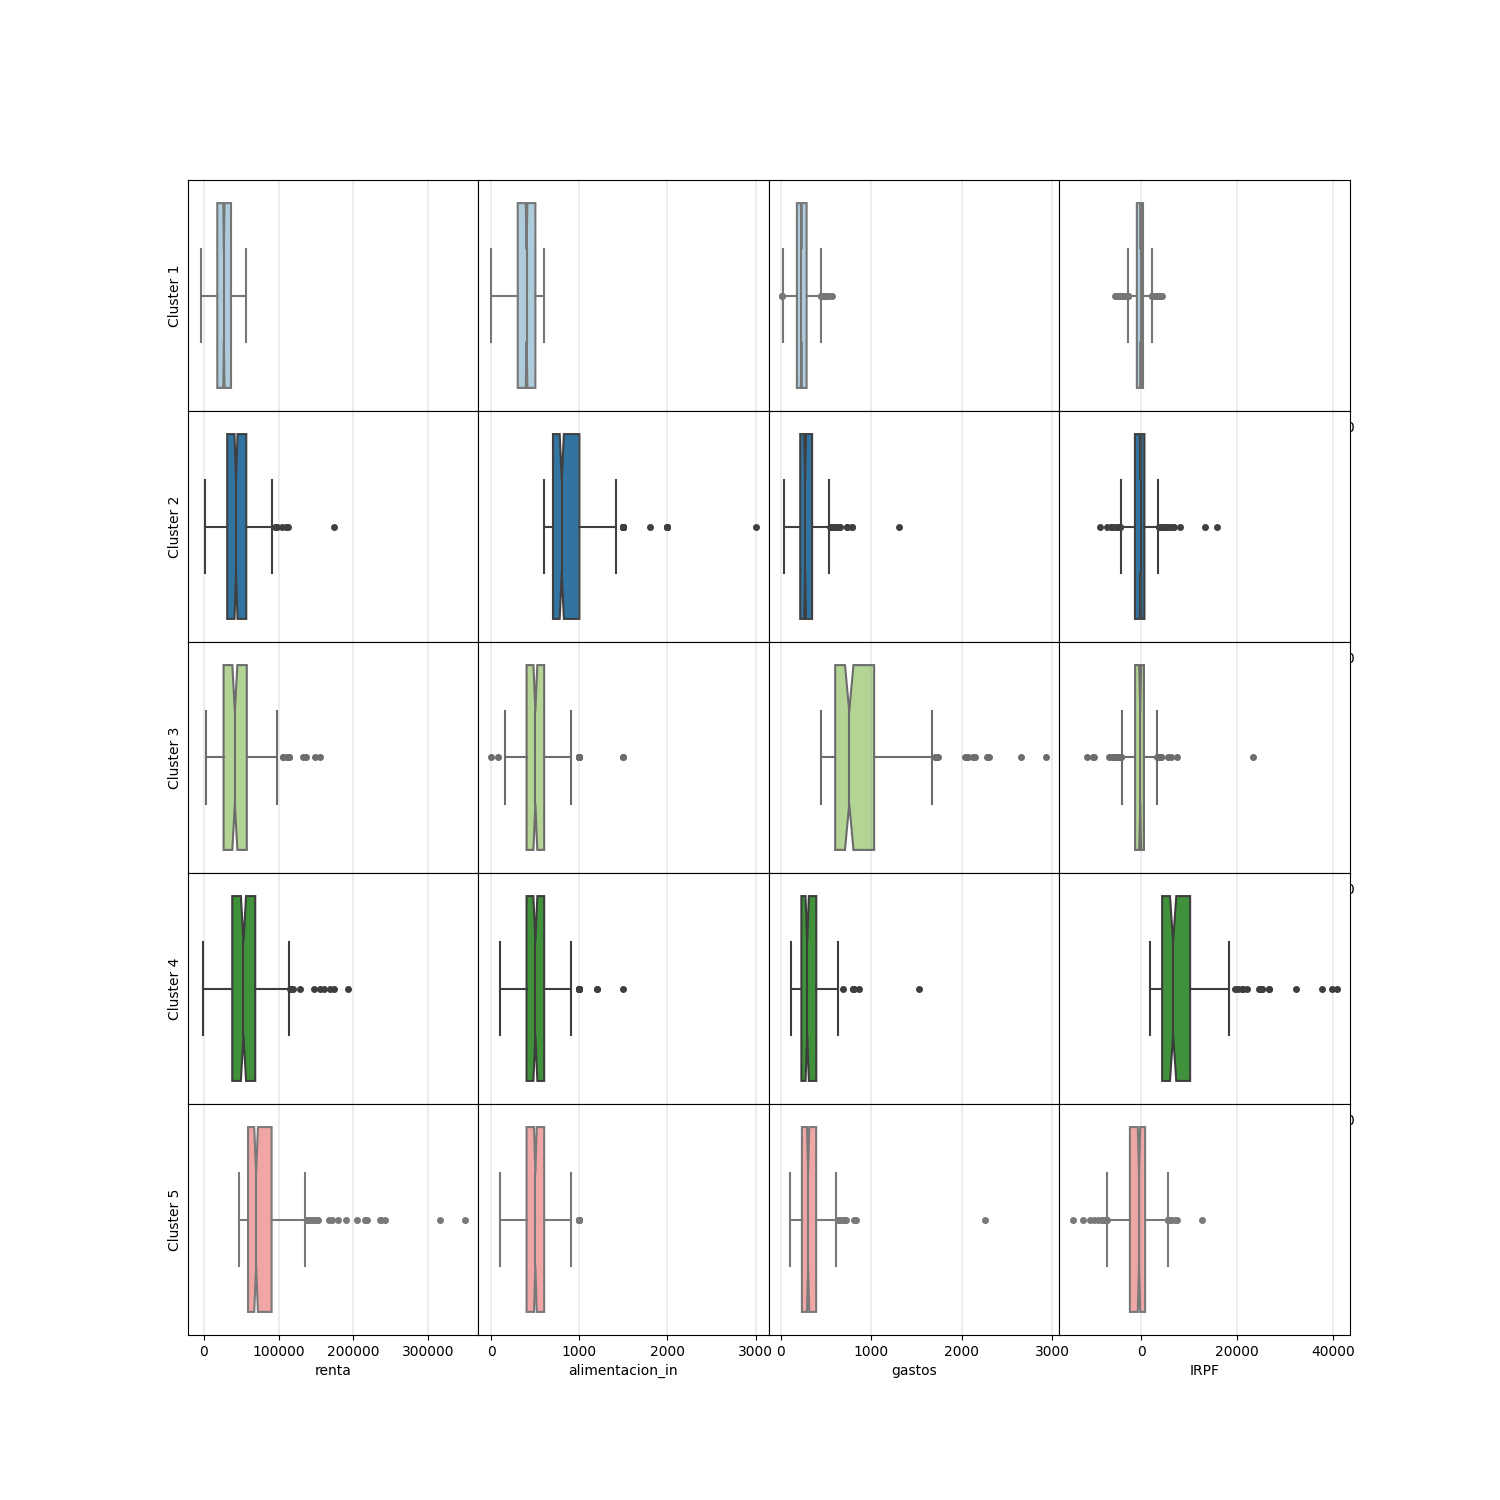
\includegraphics[scale=0.45]{caso1/spectral/boxplot.png}
\end{figure}

En \eqref{c1_boxplot} podemos observar como el cluster 3 toma valores en general mayores en gastos que los otros clusters. Esto también se observa en el cluster 4 con el IRPF y en el 2 con alimentacion in. Mientras los clusters 1 y 5 son más similares.

Notemos que al representar el boxplot la numeración de los clusters está de 1 a 5, mientras en la scatter matrix es de 0 a 4. Por tanto, hemos obtenido conclusiones análogas a las vistas en la scatter matrix.

\begin{figure}[H]
\caption{Caso 1- MDS de spectral cluster}
\label{c1_mds}
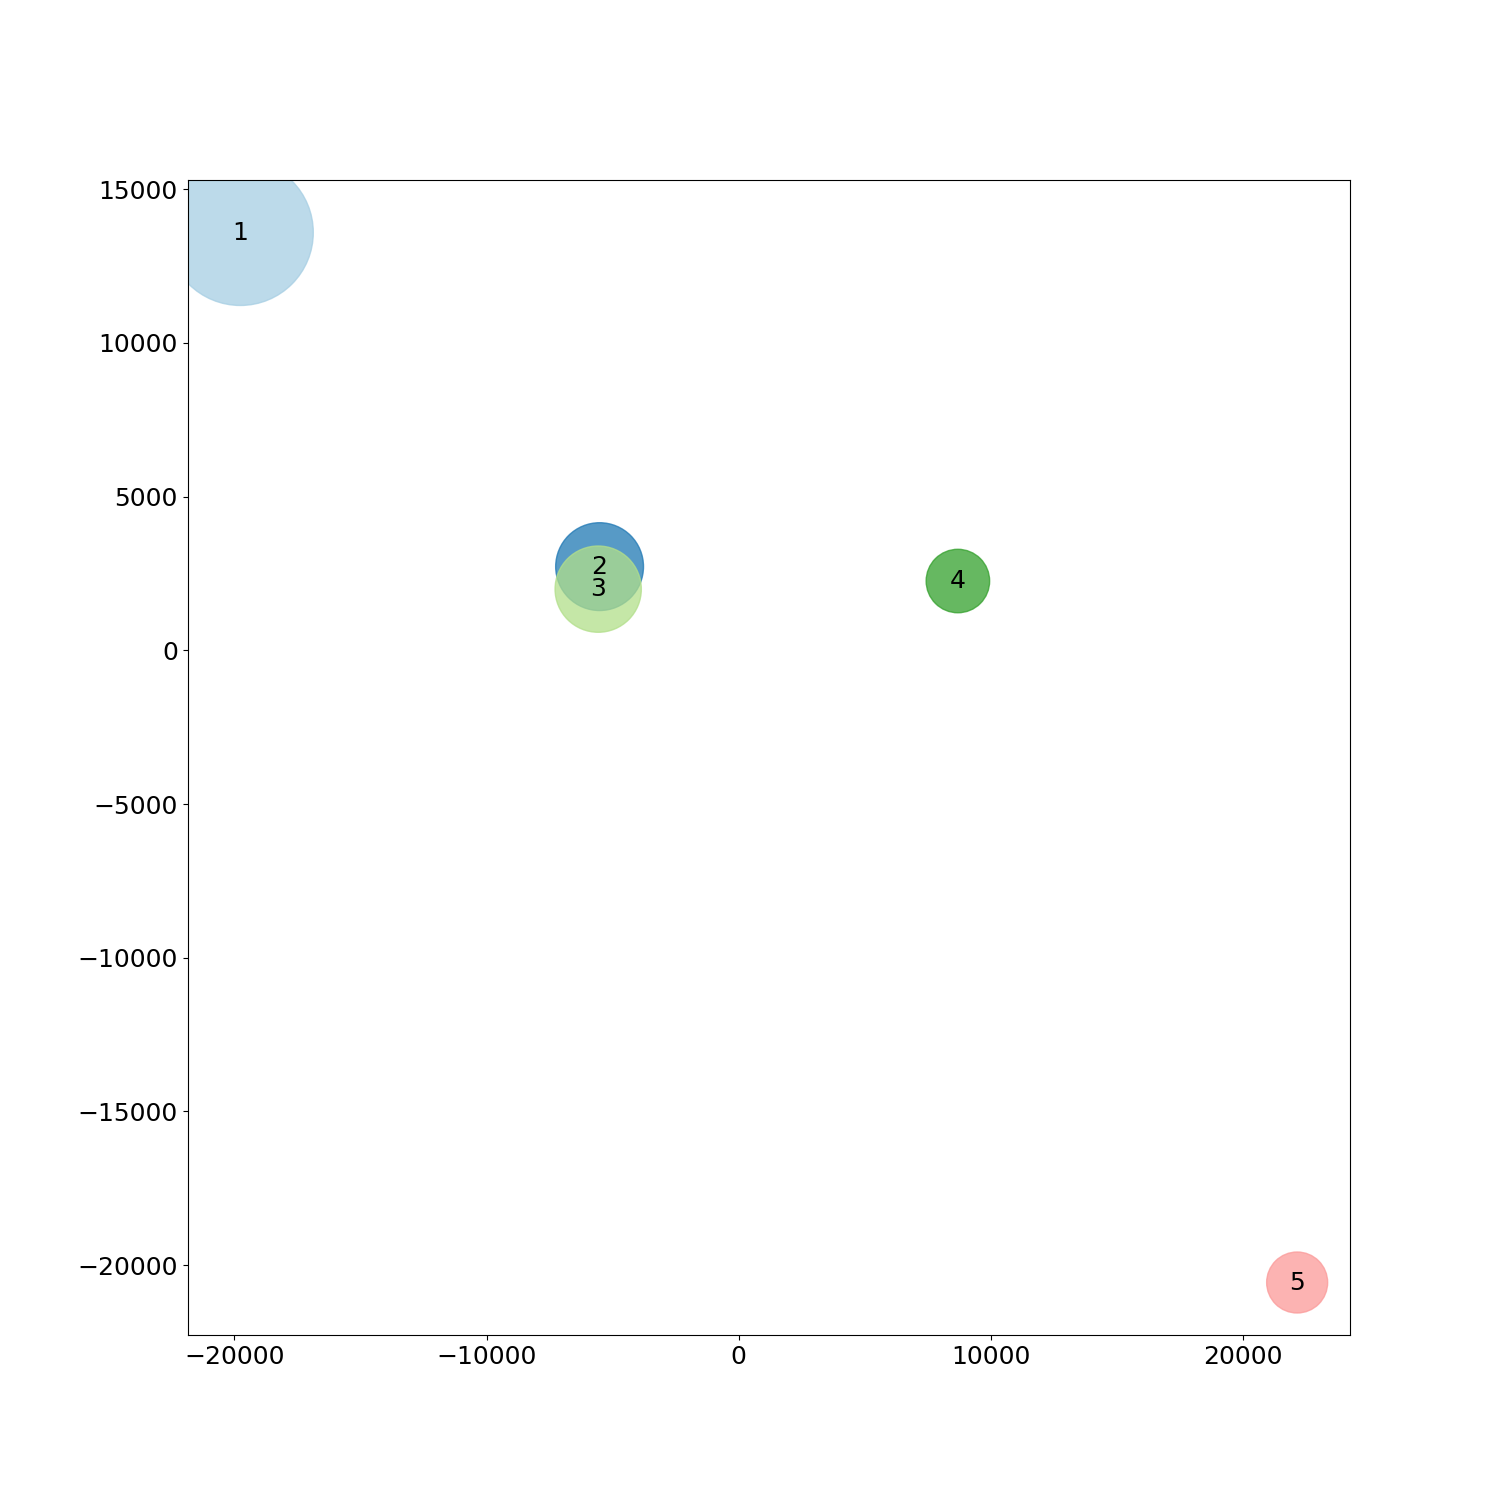
\includegraphics[scale=0.45]{caso1/spectral/mds.png}
\end{figure}

En \eqref{c1_mds} se aprecia como los clusters están considerablemente separados salvo dos que se superponen, aunque esto puede deberse a la proyección realizada. De nuevo, los clusters van de 1 a 5, pudiendo observarse desde otra perspectiva los tamaños de los clusters, cuyas proporciones coinciden con las expuestas anteriormente.


En la tabla  \eqref{tab:c1_variables} se muestran qué variables son necesarias para identificar cada cluster:

\begin{table}[H]
\centering
\caption{Caso 1 - Variables necesarias para separar el clustering en spectral cluster}
\label{tab:c1_variables}
\begin{tabular}{ccccc}
\toprule
 Cluster & renta & alimentacion in & gastos & IRPF \\
\midrule
0 & Baja & Baja & & \\
1 & & Alto & & \\
2 & & & Alto & \\
3 & & & & Alto \\
4 & Alta & Baja & & \\
\bottomrule
\end{tabular}
\end{table}
Como se aprecia en \eqref{tab:c1_variables} con una sola variable en cada cluster nos sirve para diferenciarlos entre ellos, mientras para los clusters 0 y 4 necesitamos dos para diferenciarlos entre ellos.

\section{Estudio de parámetros de DBSCAN}

Vamos a analizar el comportamiento de DBSCAN según sus parámetros principales. Para ello ejecutaremos la celda de parámetros de DBSCAN, que nos proporciona las medidas obtenidas para cada par de parámetros fijados.

\begin{table}
\centering
\caption{Caso 1 - Cambio de parámetros DBSCAN}
\label{tab:c1_dbscan}
\begin{tabular}{ccccccc}
\toprule
Algoritmo & eps & min samples & Tiempo(s) & Calinski-Harabasz & Silhouette & n clusters \\
\midrule
dbscan & 0.126 & 15 & 0.129 & 314.352 & 0.67749 & 2 \\
dbscan & 0.126 & 20 & 0.125 & 333.456 & 0.67367 & 2 \\
dbscan & 0.126 & 25 & 0.121 & 354.162 & 0.66902 & 2 \\
dbscan & 0.126 & 30 & 0.125 & 368.859 & 0.66260 & 2 \\
dbscan & 0.126 & 35 & 0.128 & 376.451 & 0.65698 & 2 \\
dbscan & 0.130 & 15 & 0.127 & 323.611 & 0.68333 & 2 \\
dbscan & 0.130 & 20 & 0.121 & 338.608 & 0.67757 & 2 \\
dbscan & 0.130 & 25 & 0.130 & 354.371 & 0.67411 & 2 \\
dbscan & 0.130 & 30 & 0.123 & 359.105 & 0.67258 & 2 \\
dbscan & 0.130 & 35 & 0.124 & 366.292 & 0.66568 & 2 \\
dbscan & 0.150 & 15 & 0.135 & 288.264 & 0.70224 & 2 \\
dbscan & 0.150 & 20 & 0.134 & 304.901 & 0.69936 & 2 \\
dbscan & 0.150 & 25 & 0.132 & 311.673 & 0.69243 & 2 \\
dbscan & 0.150 & 30 & 0.132 & 319.038 & 0.68550 & 2 \\
dbscan & 0.150 & 35 & 0.132 & 321.172 & 0.68152 & 2 \\
dbscan & 0.170 & 15 & 0.143 & 281.696 & 0.71489 & 2 \\
dbscan & 0.170 & 20 & 0.137 & 279.062 & 0.70922 & 2 \\
dbscan & 0.170 & 25 & 0.139 & 286.660 & 0.70839 & 2 \\
dbscan & 0.170 & 30 & 0.138 & 295.586 & 0.70562 & 2 \\
dbscan & 0.170 & 35 & 0.145 & 294.783 & 0.70345 & 2 \\
dbscan & 0.200 & 15 & 0.145 & 231.341 & 0.73756 & 2 \\
dbscan & 0.200 & 20 & 0.143 & 228.641 & 0.72741 & 2 \\
dbscan & 0.200 & 25 & 0.144 & 239.060 & 0.72724 & 2 \\
dbscan & 0.200 & 30 & 0.141 & 248.309 & 0.72676 & 2 \\
dbscan & 0.200 & 35 & 0.141 & 269.916 & 0.72272 & 2 \\
\bottomrule
\end{tabular}
\end{table}


Como podemos apreciar en \eqref{tab:c1_dbscan} DBSCAN siempre realiza dos clusters. El tamaño de estos es siempre similar, más del $90\%$ los ejemplos están agrupados en el cluster $0$ y los restantes están en el $-1$.

Este algoritmo no ha hecho ninguna buena agrupación en ningún caso de los probados, pese a que su silhouette es bastante alto, lo que puede ser consecuencia de que los clusters estén muy separados.

\begin{figure}[H]
\caption{Caso 1- Parámetros de DBSCAN}
\label{c1_param_dbscan}
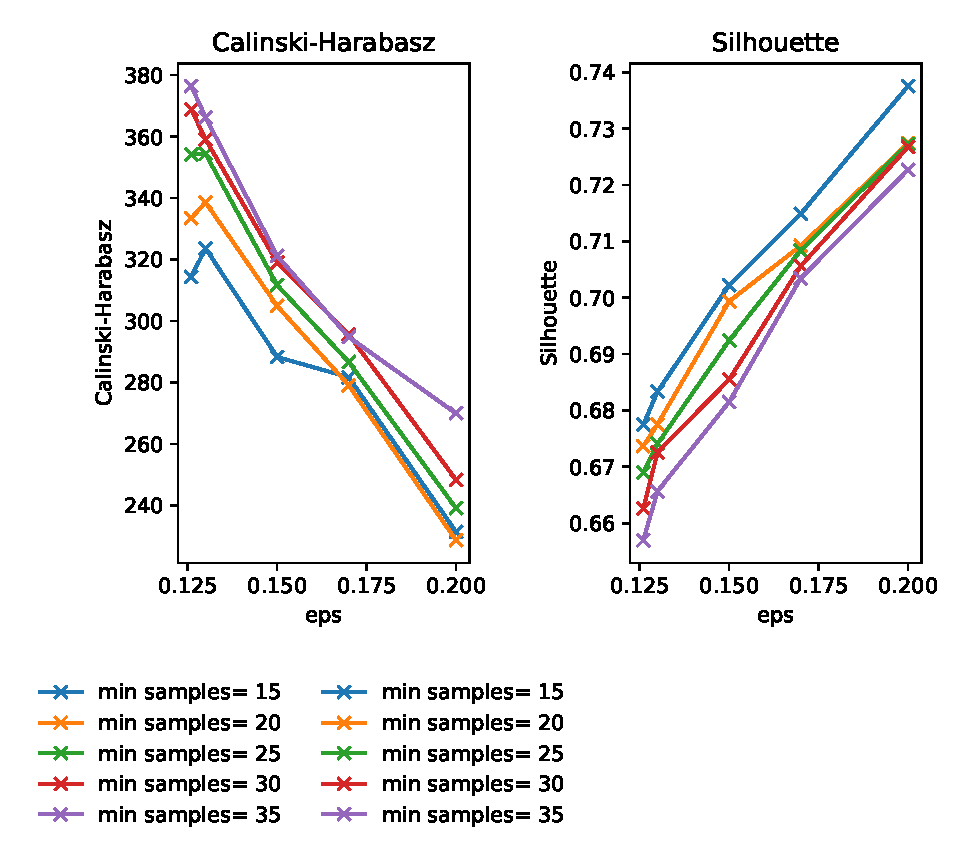
\includegraphics[scale=0.9]{caso1/parametros_dbscan.eps}
\end{figure}

No podemos interpretar demasiado Calinsk-Harabasz, ya que al no estar normalizado no sabemos si los valores dados son muy altos. Sí podemos decir que los mejores agrupamientos (que han proporcionado un valor de esta medida más alto) se han dado cuando min samples es $35$, como se puede ver en \eqref{c1_param_dbscan}.

También cabe destacar como el silhouette va creciendo conforme aumenta epsilon y calinski sube ligeramente al principio para valores bajos de min samples pero luego decrece, mientras para valores altos solo decrece. Asimismo resulta llamativo como los valores de min samples que producen valores de Calinski-harabasz más altos producen silhouettes más bajos.

Finalmente, cabe destacar como el tiempo de ejecución se incrementaba a la par que crecían los parámetros.


\section{Estudio de parámetros de Birch}

Estudiamos ahora el algoritmo Birch. Para este de nuevo se han probado distintas combinaciones de parámetros.

\begin{table}[H]
\centering
\caption{Caso 1 - Cambio de parámetros Birch}
\label{tab:c1_birch}
\begin{tabular}{ccccccc}
\toprule
Algoritmo & Branch fact & Threshold & Tiempo(s) & Calinski-Harabasz & Silhouette & n clusters \\
\midrule
birch & 15 & 0.100 & 0.087 & 336.711 & 0.48426 & 5 \\
birch & 15 & 0.150 & 0.065 & 192.073 & 0.58865 & 5 \\
birch & 15 & 0.200 & 0.060 & 206.873 & 0.60273 & 5 \\
birch & 15 & 0.250 & 0.062 &  &  & 1 \\
birch & 15 & 0.300 & 0.049 &  &  & 1 \\
birch & 20 & 0.100 & 0.147 & 173.266 & 0.58162 & 5 \\
birch & 20 & 0.150 & 0.077 & 180.842 & 0.58567 & 5 \\
birch & 20 & 0.200 & 0.046 & 206.873 & 0.60273 & 5 \\
birch & 20 & 0.250 & 0.053 &  &  & 1 \\
birch & 20 & 0.300 & 0.052 &  &  & 1 \\
birch & 25 & 0.100 & 0.153 & 312.603 & 0.49236 & 5 \\
birch & 25 & 0.150 & 0.064 & 184.304 & 0.57974 & 5 \\
birch & 25 & 0.200 & 0.045 & 206.873 & 0.60273 & 5 \\
birch & 25 & 0.250 & 0.051 &  &  & 1 \\
birch & 25 & 0.300 & 0.043 &  &  & 1 \\
birch & 30 & 0.100 & 0.136 & 292.036 & 0.52240 & 5 \\
birch & 30 & 0.150 & 0.059 & 184.304 & 0.57974 & 5 \\
birch & 30 & 0.200 & 0.066 & 206.873 & 0.60273 & 5 \\
birch & 30 & 0.250 & 0.057 &  &  & 1 \\
birch & 30 & 0.300 & 0.074 &  &  & 1 \\
birch & 35 & 0.100 & 0.129 & 355.783 & 0.42852 & 5 \\
birch & 35 & 0.150 & 0.058 & 184.304 & 0.57974 & 5 \\
birch & 35 & 0.200 & 0.061 & 206.873 & 0.60273 & 5 \\
birch & 35 & 0.250 & 0.061 &  &  & 1 \\
birch & 35 & 0.300 & 0.054 &  &  & 1 \\
\bottomrule
\end{tabular}
\end{table}

Podemos ver en \eqref{tab:c1_birch} como el algoritmo en general agrupa en $5$ clusters y obtiene resultados similares a kmeans. En general, ha hecho buenas agrupaciones a juzgar por las medidas.

Sin embargo, si miramos el tamaño de los clusters en muchas ocasiones estos se distriubuyen con un solo cluster agrupando el $90\%$ o más de los datos y los $4$ restantes el resto.

Cabe destacar que es bastante sensible a los parámetros, pues variando solo uno de ellos en ocasiones pasa de hacer 5 clusters a solo 1. Además, en estos casos no se proporcionan valores para las medidas Calinski-Harabasz y Silhouette, ya que para realizar estas es necesario tener más de un cluster.

\begin{figure}[H]
\caption{Caso 1- Parámetros de Birch}
\label{c1_param_birch}
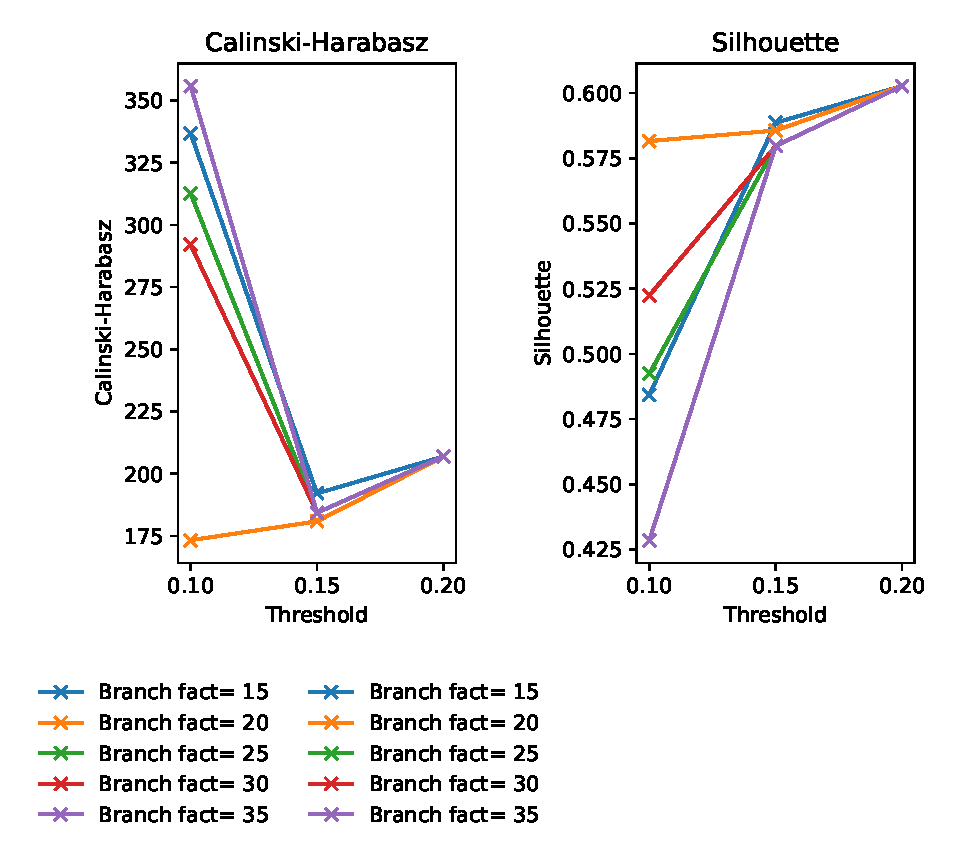
\includegraphics[scale=0.9]{caso1/parametros_birch.eps}
\end{figure}

En \eqref{c1_param_birch} se aprecia como para los valores de branch factor que producen mayor calinski-harabasz el silhouette es menor, y viceversa. Además, el silhouette siempre crece, mientras que Calinski-harabasz primero decrece y luego crece.

Teniendo en cuenta que Birch es una algoritmo que no está pensado para realizar clustering obteniendo todos los datos de una misma vez, ha generado un número de clusters razonable, pese a ser estas agrupaciones dudosas, pues los tamaños de estas son demasiado dispares.



\section{Interpretación de la segmentación}

A la vista de los resultados obtenidos, vemos que no se aprecian diferencias significativas en la renta entre las agrupaciones y no se encuentra demasiado dispersa. Esta variable por tanto no es tan relevante como otras.

No hay ninguna variable que destaque sobre otra, pero usando solamente las variables gastos, IRPF y alimentacion in podríamos diferenciar con claridad 3 clusters, y los otros dos agruparlos por descarte. Las otras variables nos sirvieron para refinar la diferenciación entre los clusters para lograr diferenciar los $5$.

Respecto a la hipótesis inicial, que las personas con propiedades alquiladas tienen mayor renta y por tanto más comodidades, en principio no parece cierta, pues la renta no ha sido una variable significativa respecto a la que dividir y otros factores son más influyentes.




